\newpage
\section{Protocolli tra entità attive del sistema}
Seguendo il modello IDM un parametro importante da considerare per l'avanzamento delle entità passive è la distanza tra l'entità stessa e la fine della traiettoria del mezzo che si trova davanti o che l'entità potrebbe trovarsi davanti a seguito di uscite da ingressi o cambi corsia di altri mezzi che si trovano davanti al mezzo interessato. Tutta la logica dell'avanzamento viene quindi basata sul calcolo delle distanze ai mezzi antecedenti il mezzo interessato. Il calcolo di questa distanza deve essere fatto in relazione alla posizione del mezzo che copriva nel quanto di tempo antecedente al quanto di tempo in cui viene effettuato l'aggiornamento della nuova posizione (anche per questo motivo il $\Delta$ del sistema non può assumere valori troppo grandi). Ribadendo quali sono le entità attive del sistema: incroci, strade principali, strade d'ingresso è necessario stabilire dei protocolli di comunicazione tra le entità. In particolare conviene dapprima fissare un ordine di esecuzione per le entità attive:

\begin{figure}[H] % Example image
\center{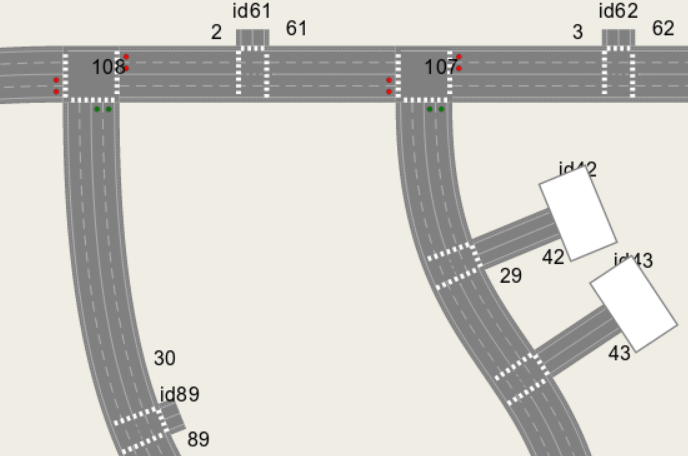
\includegraphics[width=0.9\linewidth]{EsempioMappa}}
\caption{Un frammento di mappa di un quartiere.}
\label{fig:Un frammento di mappa di un quartiere}
\end{figure}

Come da esempio in \ref{fig:Un frammento di mappa di un quartiere} si può notare che una strada principale è limitata al più da 2 incroci e una strada può o meno avere degli ingressi. Considerando questo modello conviene stabilire una dipendenza tra le strade principali e gli incroci e una dipendenza tra gli ingressi e le strade principali. \\
Una strada principale può iniziare a calcolare gli aggiornamenti di posizione delle entità solo dopo che gli incroci da cui è limitata hanno eseguito lo spostamento delle loro entità; questa dipendenza porta al seguente vantaggio: quando una strada principale deve eseguire l'avanzamento delle entità al $\Delta$ di sistema conosce lo stato aggiornato delle entità nell'incrocio e inoltre un incrocio potrà operare in un certo quanto di tempo conoscendo tutte le entità che dovranno essere spostate, dato che l'urbana non potrà demandare all'incrocio la gestione dello spostamento di una nuova entità se non dal quanto di tempo successivo. Analogamente il vantaggio che si ricava nel far eseguire gli spostamenti delle entità alle strade principali prima delle strade di ingresso è dovuto al fatto che una entità strada d'ingresso potrà conoscere lo stato aggiornato della strada principale permettendo quindi un sistema di gestione delle precedenze per le macchine in uscita dagli ingressi in assenza di semafori.

\subsection{Protocollo di avanzamento e aggiornamento dello stato delle entità}
In questa sezione viene esposta e analizzata la struttura di un'entità attiva. Innanzitutto occorre predisporre una "mailbox" per ogni entità attiva. Una mailbox è una entità reattiva di tipo risorsa che ha il compito di contenere lo stato delle entità che la rispettiva entità attiva ha in gestione; attraverso la mailbox le entità attive possono comunicare tra loro notificando inserimenti e/o rimozioni di entità da spostare, informando altre entità attive delle posizioni occupate dalle entità passive, dello stato della risorsa stessa ad esempio nel caso di incroci la risorsa dovrà rendere disponibile un'interfaccia per comunicare se il semaforo è verde o rosso, ecc.

\begin{codiceada}[caption={Template-Code entità attiva}, label=template-code]
loop
	synchronization_with_delta;
	mailbox.update_entity_status;	
	update_view;	
	move_entity;
end loop;
\end{codiceada}
\\
Dove:
\begin{itemize}
\item \textit{synchronization\_with\_delta} è la procedura utilizzata per permettere all'entità di entrare in sincronizzazione con il sistema al quanto di tempo successivo;
\item \textit{mailbox.update\_entity\_status} è la procedura utilizzata per aggiornare la posizione delle entità calcolate al quanto di tempo precedente; \item \textit{update\_view} è la procedura utilizzata per inviare al web server le posizioni delle entità aggiornate al nuovo delta;
\item \textit{move\_entity} è la procedura utilizzata per spostare le enitità in gestione all'entità attiva corrente.
\end{itemize}

A seconda poi del tipo di entità occorrerà eseguire delle attese per favorire la gestione delle precedenze e per facilitare la consistenza dello stato della risorsa in un preciso quanto di tempo. \\
Quindi a seconda del tipo di entità attiva sarà necessario integrare al template di codice in \ref{template-code} le seguenti strutture:
\begin{itemize}
\item per gli incroci:\\
\begin{codiceada}[caption={Template-Code incroci}, label=template-code-incroci]
loop
	-- same code rows: [2-5]
	wake_up_strade_principali;
	move_entity;
end loop;
\end{codiceada}
\\
Dove:
\begin{itemize}
\item \textit{wake\_up\_strade\_principali} è la procedura utilizzata per comunicare ad ogni strada principale interessata nell'incrocio che l'incrocio ha terminato l'aggiornamento delle entità per il quanto di tempo del sistema.
\end{itemize}
\item per le strade principali:\\
\begin{codiceada}[caption={Template-Code strade principali}, label=template-code-principali]
loop
	-- same code rows: [2-4]
	mailbox.wait_incroci;	
	move_entity;
	mailbox.finish_delta_updated;
end loop;
\end{codiceada}
\\
Dove:
\begin{itemize}
\item \textit{mailbox.wait\_incroci} è la procedura utilizzata dalla strada prinicipale per aspettare la terminazione dell'aggiornamento delle entità degli incroci interessati relativamente al quanto di tempo del sistema.
\end{itemize}
\item per le strade d'ingresso:\\
\begin{codiceada}[caption={Template-Code strade ingresso}, label=template-code-ingresso]
loop
	-- same code rows: [2-4]
	mailbox_urbana.wait_urbana_finish_delta;	
	move_entity;
end loop;
\end{codiceada}
\\
Dove:
\begin{itemize}
\item \textit{mailbox\_urbana.wait\_urbana\_finish\_delta	
} è la procedura utilizzata dalla strada d'ingresso per aspettare la terminazione dell'aggiornamento delle entità della strada principale alla quale l'ingresso si riferisce relativamente al quanto di tempo del sistema. Vale la pena qui dire che una strada d'ingresso apparterrà sempre allo stesso quartiere al quale appartiene la strada principale alla quale l'ingresso si riferisce.
\end{itemize}
\end{itemize}

\subsubsection{Gestione dello spostamento delle entità per le strade d'ingresso}
Vista la struttura disposta da un task di tipo strada ingresso, vedi \ref{template-code-ingresso}, qui in questa sezione viene analizzata la modalità dello spostamento delle entità passive da parte di un'entità di tipo ingresso.\\
Nel modello della mappa ciò che viene classificato come strada d'ingresso dispone di una corsia per senso di marcia, un marciapiede e una pista ciclabile.\\
Quindi di seguito viene riportato il sistema che si occupa dello spostamento delle entità degli ingressi e il protocollo di interazione con la strada principale alla quale l'ingresso si riferisce:
\begin{enumerate}
\item per questa tipologia di entità attiva possono essere spostati indifferentemente mezzi, bici o pedoni senza un ordine prioritario;
\item un'entità passiva viene inserita nel sistema attraverso le strade d'ingresso; occorre controllare se nella mailbox dell'ingresso sono state inserite delle entità per cui occorre iniziare lo spostamento; se vi sono delle entità occorre trasferirle dalla lista temporanea della mailbox alla lista che si occupa della gestione dello spostamento delle entità. La lista temporanea è necessaria dato che l'inserimento di nuove entità nella mailbox può avvenire in qualunque momento; sarà poi il task a decidere il momento per iniziare a spostare le nuove entità;
\item la strada d'ingresso può essere percorsa secondo il verso d'uscita della strada, oppure secondo il verso d'entrata della strada; considerando entrambi i versi di percorrenza l'ordine con cui le entità possono essere spostate può essere eseguito sia, dall'entità più vicina alla fine del verso di percorrenza all'entità inserita a inizio del verso di percorrenza, che viceversa; supponiamo che venga scelto l'ordine dall'entità più distante dalla fine del verso di percorrenza all'entità più vicina alla fine del verso di percorrenza;
\item un'entità passiva, seguendo il suo verso di percorrenza, può essere preceduta da un'altra entità passiva oppure semplicemente dalla sola limitazione della fine della strada d'ingresso;
\item se l'entità passiva presenta davanti un'altra entità allora il calcolo della distanza dall'entità precedente sarà una conoscenza disponibile localmente nella mailbox della strada d'ingresso; mentre se l'entità passiva non è preceduta da nessuna altra entità occorrerà controllare la posizione delle entità in uscita dagli ingressi per le entità che seguono il verso di percorrenza in uscita dagli ingressi; mentre seguendo il verso di percorrenza in entrata dagli ingressi non ha alcuna importanza imporre un limite dato che l'entità ha concluso il percorso ed è in procinto di uscire dal sistema.
Per controllare la posizione delle entità in uscita dagli ingressi, il task potrà controllare l'avanzamento delle entità "cedute" alla strada principale direttamente dalla propria mailbox; infatti il protocollo di comunicazione tra task della strada principale e task ingresso prevede che il task della strada prinicipale aggiorni le mailbox degli ingressi in merito all'avanzamento delle entità in uscita dagli ingressi fintanto che le entità interessate non siano uscite completamente dall'ingresso considerando la lunghezza dell'entità stessa;
\item per le macchine che seguono il verso di percorrenza in uscita dagli ingressi occorre considerare se la posizione dell'entità raggiunge la lunghezza dell'ingresso con l'aggiornamento della posizione alla fine del quanto del sistema in corso d'opera. Se l'entità alla fine del quanto, quindi dopo l'aggiornamento della nuova posizione raggiunge la fine della lunghezza dell'ingresso sarà necessario aggiungere l'entità nella mailbox della strada principale; questa operazione viene effettuata prima della nuova sincronizzazione da parte del task ingresso stesso, affinchè la strada principale quando rieffettua la sincronizzazione, che sarà dopo l'esecuzione delle operazioni degli ingressi, troverà nella mailbox la nuova entità da spostare e la troverà in posizione 0 nella traiettoria che dovrà intraprendere (gestita dalla strada principale); l'ingresso quindi rimuoverà l'entità che ha raggiunto la fine della strada d'ingresso dato che questa entità è stata inserita nella mailbox della strada principale e quindi dal prossimo quanto sarà in gestione dal task della strada principale interessata. La traiettoria che l'entità dovrà intraprendere deve essere calcolata dall'ingresso stesso, al fine di permettere alla strada principale di trovare un'entità da spostare correttamente configurata; il calcolo della traiettoria da intraprendere deve avvenire interrogando il servizio di locazione delle entità disponibile in ogni quartiere. Tale servizio contiene tutti i percorsi e la storia del percorso eseguito di tutte le entità istanziate nel quartiere stesso. Un'entità quindi prima di essere inserita nella mailbox degli ingressi presenta già il percorso completamente configurato presso il gestore del servizio di locazione delle entità del quartiere. Il calcolo della traiettoria da intraprendere si basa sulle convenzioni utilizzate per la creazione della mappa.
\end{enumerate}
Il protocollo di avanzamento delle entità per gli ingressi prevede un ordine FIFO nell'avanzamento delle entità senza prevedere possibilità di sorpassi o attraversamenti pedonali; se l'entità è un veicolo allora questo potrà essere preceduto solamente dalla fine della strada o da un veicolo dello stesso tipo; analogamente per le entità di tipo pedone e bici. 

\subsubsection{Gestione dello spostamento delle entità per le strade principali}
\subsubsection{Gestione dello spostamento delle entità per gli incroci}
